\documentclass[12pt,letterpaper]{article}
\usepackage[letterpaper,left=0.62in,right=0.62in,top=0.75in,bottom=0.65in,headheight=14pt,headsep=0.17in,footskip=0.32in]{geometry}
\usepackage[T1]{fontenc}
\usepackage{lmodern}
\pdfmapfile{+lm.map}
\usepackage{tikz}
\usepackage{fancyhdr}
\definecolor{Rfill}{RGB}{251,227,225}
\definecolor{Bfill}{RGB}{223,235,251}
\definecolor{Yfill}{RGB}{255,247,203}
\pagestyle{fancy}
\fancyhf{}
\renewcommand{\headrulewidth}{0pt}
\renewcommand{\footrulewidth}{0pt}
\setlength{\parindent}{0pt}
\setlength{\parskip}{0pt}
\setlength{\emergencystretch}{2em}
\raggedbottom
\sffamily
\fancyhead[L]{\fontsize{10.5}{12}\selectfont Week 16 / Three-color triangles / K--1}
\fancyfoot[L]{\fontsize{9}{11}\selectfont Bellingham Math Circle / Week 16 / F16-K-v2}
\fancyfoot[R]{\fontsize{9}{11}\selectfont\thepage}
\begin{document}
\fontsize{15}{19}\selectfont
Put one R, B, or Y counter on every dot. Keep the corner letters. Each outside side allows only the letters beside it. A little triangle has no lines inside.\par\vspace{0.23in}
\textbf{Problem 1:} Fill the dots with counters. Move the counters to put a little triangle with R, B, and Y in each of the four places, one at a time.\par\vspace{0.16in}
\begin{center}
\begin{tikzpicture}[x=1in,y=1in,line cap=round,line join=round]
\path[use as bounding box] (-0.63,-0.64) rectangle (5.8800,4.7966);
\draw[line width=0.8pt] (0.0000,0.0000) -- (1.3125,2.2733);
\draw[line width=0.8pt] (0.0000,0.0000) -- (2.6250,0.0000);
\draw[line width=0.8pt] (1.3125,2.2733) -- (2.6250,4.5466);
\draw[line width=0.8pt] (1.3125,2.2733) -- (2.6250,0.0000);
\draw[line width=0.8pt] (1.3125,2.2733) -- (3.9375,2.2733);
\draw[line width=0.8pt] (2.6250,4.5466) -- (3.9375,2.2733);
\draw[line width=0.8pt] (2.6250,0.0000) -- (3.9375,2.2733);
\draw[line width=0.8pt] (2.6250,0.0000) -- (5.2500,0.0000);
\draw[line width=0.8pt] (3.9375,2.2733) -- (5.2500,0.0000);
\node[circle,draw,line width=0.8pt,fill=Rfill,minimum size=0.30in,inner sep=0pt,font=\sffamily\bfseries\fontsize{11.5}{12}\selectfont] at (0.0000,0.0000) {R};
\draw[line width=0.8pt,fill=white] (2.6250,0.0000) circle[radius=0.092in];
\node[circle,draw,line width=0.8pt,fill=Bfill,minimum size=0.30in,inner sep=0pt,font=\sffamily\bfseries\fontsize{11.5}{12}\selectfont] at (5.2500,0.0000) {B};
\draw[line width=0.8pt,fill=white] (1.3125,2.2733) circle[radius=0.092in];
\draw[line width=0.8pt,fill=white] (3.9375,2.2733) circle[radius=0.092in];
\node[circle,draw,line width=0.8pt,fill=Yfill,minimum size=0.30in,inner sep=0pt,font=\sffamily\bfseries\fontsize{11.5}{12}\selectfont] at (2.6250,4.5466) {Y};
\node[rotate=60,font=\sffamily\fontsize{11}{12}\selectfont] at (0.9825,2.4333) {R or Y};
\node[rotate=-60,font=\sffamily\fontsize{11}{12}\selectfont] at (4.2675,2.4333) {B or Y};
\node[font=\sffamily\fontsize{11}{12}\selectfont] at (2.6250,-0.48) {R or B};
\end{tikzpicture}
\end{center}
\newpage
\textbf{Problem 2:} Can you fill the dots without making a little triangle with R, B, and Y?\par\vspace{0.16in}
\begin{center}
\begin{tikzpicture}[x=1in,y=1in,line cap=round,line join=round]
\path[use as bounding box] (-0.63,-0.64) rectangle (5.8800,4.7966);
\draw[line width=0.8pt] (0.0000,0.0000) -- (0.8750,1.5155);
\draw[line width=0.8pt] (0.0000,0.0000) -- (1.7500,0.0000);
\draw[line width=0.8pt] (0.8750,1.5155) -- (1.7500,3.0311);
\draw[line width=0.8pt] (0.8750,1.5155) -- (1.7500,0.0000);
\draw[line width=0.8pt] (0.8750,1.5155) -- (2.6250,1.5155);
\draw[line width=0.8pt] (1.7500,3.0311) -- (2.6250,4.5466);
\draw[line width=0.8pt] (1.7500,3.0311) -- (2.6250,1.5155);
\draw[line width=0.8pt] (1.7500,3.0311) -- (3.5000,3.0311);
\draw[line width=0.8pt] (2.6250,4.5466) -- (3.5000,3.0311);
\draw[line width=0.8pt] (1.7500,0.0000) -- (2.6250,1.5155);
\draw[line width=0.8pt] (1.7500,0.0000) -- (3.5000,0.0000);
\draw[line width=0.8pt] (2.6250,1.5155) -- (3.5000,3.0311);
\draw[line width=0.8pt] (2.6250,1.5155) -- (3.5000,0.0000);
\draw[line width=0.8pt] (2.6250,1.5155) -- (4.3750,1.5155);
\draw[line width=0.8pt] (3.5000,3.0311) -- (4.3750,1.5155);
\draw[line width=0.8pt] (3.5000,0.0000) -- (4.3750,1.5155);
\draw[line width=0.8pt] (3.5000,0.0000) -- (5.2500,0.0000);
\draw[line width=0.8pt] (4.3750,1.5155) -- (5.2500,0.0000);
\node[circle,draw,line width=0.8pt,fill=Rfill,minimum size=0.30in,inner sep=0pt,font=\sffamily\bfseries\fontsize{11.5}{12}\selectfont] at (0.0000,0.0000) {R};
\draw[line width=0.8pt,fill=white] (1.7500,0.0000) circle[radius=0.092in];
\draw[line width=0.8pt,fill=white] (3.5000,0.0000) circle[radius=0.092in];
\node[circle,draw,line width=0.8pt,fill=Bfill,minimum size=0.30in,inner sep=0pt,font=\sffamily\bfseries\fontsize{11.5}{12}\selectfont] at (5.2500,0.0000) {B};
\draw[line width=0.8pt,fill=white] (0.8750,1.5155) circle[radius=0.092in];
\draw[line width=0.8pt,fill=white] (2.6250,1.5155) circle[radius=0.092in];
\draw[line width=0.8pt,fill=white] (4.3750,1.5155) circle[radius=0.092in];
\draw[line width=0.8pt,fill=white] (1.7500,3.0311) circle[radius=0.092in];
\draw[line width=0.8pt,fill=white] (3.5000,3.0311) circle[radius=0.092in];
\node[circle,draw,line width=0.8pt,fill=Yfill,minimum size=0.30in,inner sep=0pt,font=\sffamily\bfseries\fontsize{11.5}{12}\selectfont] at (2.6250,4.5466) {Y};
\node[rotate=60,font=\sffamily\fontsize{11}{12}\selectfont] at (0.9825,2.4333) {R or Y};
\node[rotate=-60,font=\sffamily\fontsize{11}{12}\selectfont] at (4.2675,2.4333) {B or Y};
\node[font=\sffamily\fontsize{11}{12}\selectfont] at (2.6250,-0.48) {R or B};
\end{tikzpicture}
\end{center}
\newpage
\textbf{Problem 3:} Fill the dots to make as many little triangles with R, B, and Y as you can.\par\vspace{0.16in}
\begin{center}
\begin{tikzpicture}[x=1in,y=1in,line cap=round,line join=round]
\path[use as bounding box] (-0.63,-0.64) rectangle (5.8800,4.7966);
\draw[line width=0.8pt] (0.0000,0.0000) -- (0.8750,1.5155);
\draw[line width=0.8pt] (0.0000,0.0000) -- (1.7500,0.0000);
\draw[line width=0.8pt] (0.8750,1.5155) -- (1.7500,3.0311);
\draw[line width=0.8pt] (0.8750,1.5155) -- (1.7500,0.0000);
\draw[line width=0.8pt] (0.8750,1.5155) -- (2.6250,1.5155);
\draw[line width=0.8pt] (1.7500,3.0311) -- (2.6250,4.5466);
\draw[line width=0.8pt] (1.7500,3.0311) -- (2.6250,1.5155);
\draw[line width=0.8pt] (1.7500,3.0311) -- (3.5000,3.0311);
\draw[line width=0.8pt] (2.6250,4.5466) -- (3.5000,3.0311);
\draw[line width=0.8pt] (1.7500,0.0000) -- (2.6250,1.5155);
\draw[line width=0.8pt] (1.7500,0.0000) -- (3.5000,0.0000);
\draw[line width=0.8pt] (2.6250,1.5155) -- (3.5000,3.0311);
\draw[line width=0.8pt] (2.6250,1.5155) -- (3.5000,0.0000);
\draw[line width=0.8pt] (2.6250,1.5155) -- (4.3750,1.5155);
\draw[line width=0.8pt] (3.5000,3.0311) -- (4.3750,1.5155);
\draw[line width=0.8pt] (3.5000,0.0000) -- (4.3750,1.5155);
\draw[line width=0.8pt] (3.5000,0.0000) -- (5.2500,0.0000);
\draw[line width=0.8pt] (4.3750,1.5155) -- (5.2500,0.0000);
\node[circle,draw,line width=0.8pt,fill=Rfill,minimum size=0.30in,inner sep=0pt,font=\sffamily\bfseries\fontsize{11.5}{12}\selectfont] at (0.0000,0.0000) {R};
\draw[line width=0.8pt,fill=white] (1.7500,0.0000) circle[radius=0.092in];
\draw[line width=0.8pt,fill=white] (3.5000,0.0000) circle[radius=0.092in];
\node[circle,draw,line width=0.8pt,fill=Bfill,minimum size=0.30in,inner sep=0pt,font=\sffamily\bfseries\fontsize{11.5}{12}\selectfont] at (5.2500,0.0000) {B};
\draw[line width=0.8pt,fill=white] (0.8750,1.5155) circle[radius=0.092in];
\draw[line width=0.8pt,fill=white] (2.6250,1.5155) circle[radius=0.092in];
\draw[line width=0.8pt,fill=white] (4.3750,1.5155) circle[radius=0.092in];
\draw[line width=0.8pt,fill=white] (1.7500,3.0311) circle[radius=0.092in];
\draw[line width=0.8pt,fill=white] (3.5000,3.0311) circle[radius=0.092in];
\node[circle,draw,line width=0.8pt,fill=Yfill,minimum size=0.30in,inner sep=0pt,font=\sffamily\bfseries\fontsize{11.5}{12}\selectfont] at (2.6250,4.5466) {Y};
\node[rotate=60,font=\sffamily\fontsize{11}{12}\selectfont] at (0.9825,2.4333) {R or Y};
\node[rotate=-60,font=\sffamily\fontsize{11}{12}\selectfont] at (4.2675,2.4333) {B or Y};
\node[font=\sffamily\fontsize{11}{12}\selectfont] at (2.6250,-0.48) {R or B};
\end{tikzpicture}
\end{center}
\newpage
\textbf{Problem 4:} Keep every printed letter. Fill the empty dots to make as many little triangles with R, B, and Y as you can.\par\vspace{0.16in}
\begin{center}
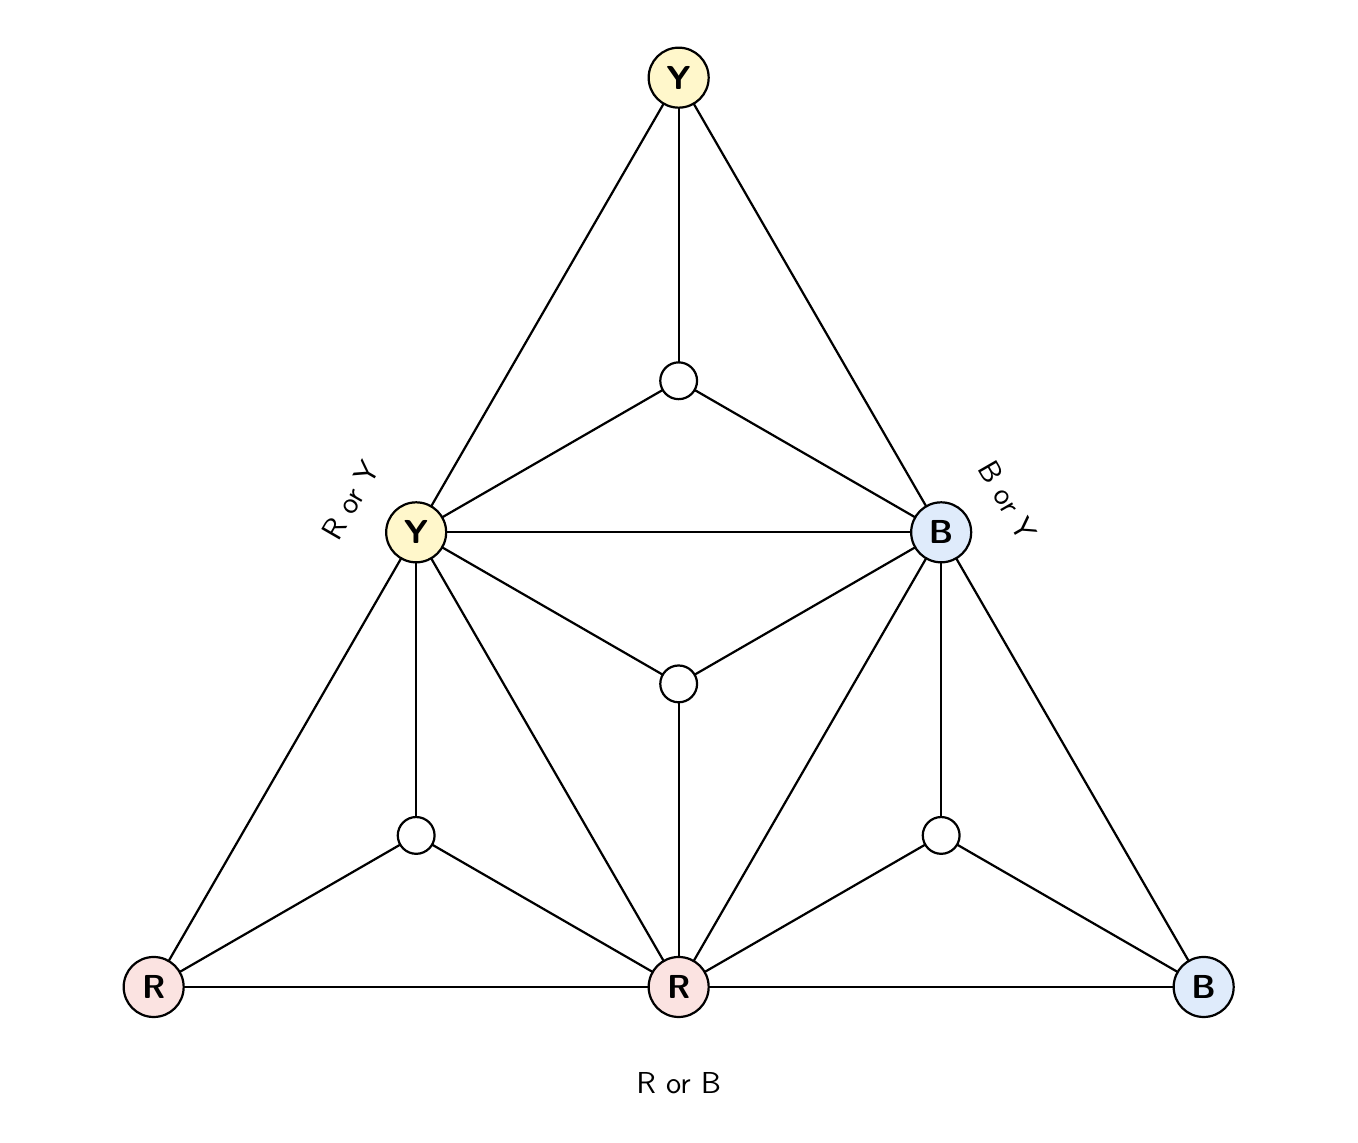
\begin{tikzpicture}[x=1in,y=1in,line cap=round,line join=round]
\path[use as bounding box] (-0.63,-0.64) rectangle (5.8800,4.7966);
\draw[line width=0.8pt] (0.0000,0.0000) -- (1.3125,2.2733);
\draw[line width=0.8pt] (0.0000,0.0000) -- (2.6250,0.0000);
\draw[line width=0.8pt] (0.0000,0.0000) -- (1.3125,0.7578);
\draw[line width=0.8pt] (1.3125,2.2733) -- (2.6250,4.5466);
\draw[line width=0.8pt] (1.3125,2.2733) -- (2.6250,0.0000);
\draw[line width=0.8pt] (1.3125,2.2733) -- (3.9375,2.2733);
\draw[line width=0.8pt] (1.3125,2.2733) -- (1.3125,0.7578);
\draw[line width=0.8pt] (1.3125,2.2733) -- (2.6250,1.5155);
\draw[line width=0.8pt] (1.3125,2.2733) -- (2.6250,3.0311);
\draw[line width=0.8pt] (2.6250,4.5466) -- (3.9375,2.2733);
\draw[line width=0.8pt] (2.6250,4.5466) -- (2.6250,3.0311);
\draw[line width=0.8pt] (2.6250,0.0000) -- (3.9375,2.2733);
\draw[line width=0.8pt] (2.6250,0.0000) -- (5.2500,0.0000);
\draw[line width=0.8pt] (2.6250,0.0000) -- (1.3125,0.7578);
\draw[line width=0.8pt] (2.6250,0.0000) -- (2.6250,1.5155);
\draw[line width=0.8pt] (2.6250,0.0000) -- (3.9375,0.7578);
\draw[line width=0.8pt] (3.9375,2.2733) -- (5.2500,0.0000);
\draw[line width=0.8pt] (3.9375,2.2733) -- (2.6250,1.5155);
\draw[line width=0.8pt] (3.9375,2.2733) -- (3.9375,0.7578);
\draw[line width=0.8pt] (3.9375,2.2733) -- (2.6250,3.0311);
\draw[line width=0.8pt] (5.2500,0.0000) -- (3.9375,0.7578);
\node[circle,draw,line width=0.8pt,fill=Rfill,minimum size=0.30in,inner sep=0pt,font=\sffamily\bfseries\fontsize{11.5}{12}\selectfont] at (0.0000,0.0000) {R};
\node[circle,draw,line width=0.8pt,fill=Rfill,minimum size=0.30in,inner sep=0pt,font=\sffamily\bfseries\fontsize{11.5}{12}\selectfont] at (2.6250,0.0000) {R};
\node[circle,draw,line width=0.8pt,fill=Bfill,minimum size=0.30in,inner sep=0pt,font=\sffamily\bfseries\fontsize{11.5}{12}\selectfont] at (5.2500,0.0000) {B};
\node[circle,draw,line width=0.8pt,fill=Yfill,minimum size=0.30in,inner sep=0pt,font=\sffamily\bfseries\fontsize{11.5}{12}\selectfont] at (1.3125,2.2733) {Y};
\node[circle,draw,line width=0.8pt,fill=Bfill,minimum size=0.30in,inner sep=0pt,font=\sffamily\bfseries\fontsize{11.5}{12}\selectfont] at (3.9375,2.2733) {B};
\node[circle,draw,line width=0.8pt,fill=Yfill,minimum size=0.30in,inner sep=0pt,font=\sffamily\bfseries\fontsize{11.5}{12}\selectfont] at (2.6250,4.5466) {Y};
\draw[line width=0.8pt,fill=white] (1.3125,0.7578) circle[radius=0.092in];
\draw[line width=0.8pt,fill=white] (2.6250,1.5155) circle[radius=0.092in];
\draw[line width=0.8pt,fill=white] (3.9375,0.7578) circle[radius=0.092in];
\draw[line width=0.8pt,fill=white] (2.6250,3.0311) circle[radius=0.092in];
\node[rotate=60,font=\sffamily\fontsize{11}{12}\selectfont] at (0.9825,2.4333) {R or Y};
\node[rotate=-60,font=\sffamily\fontsize{11}{12}\selectfont] at (4.2675,2.4333) {B or Y};
\node[font=\sffamily\fontsize{11}{12}\selectfont] at (2.6250,-0.48) {R or B};
\end{tikzpicture}
\end{center}
\newpage
\textbf{Problem 5:} Make just one little triangle with R, B, and Y. Move the counters to put it in as many different places as you can.\par\vspace{0.16in}
\begin{center}
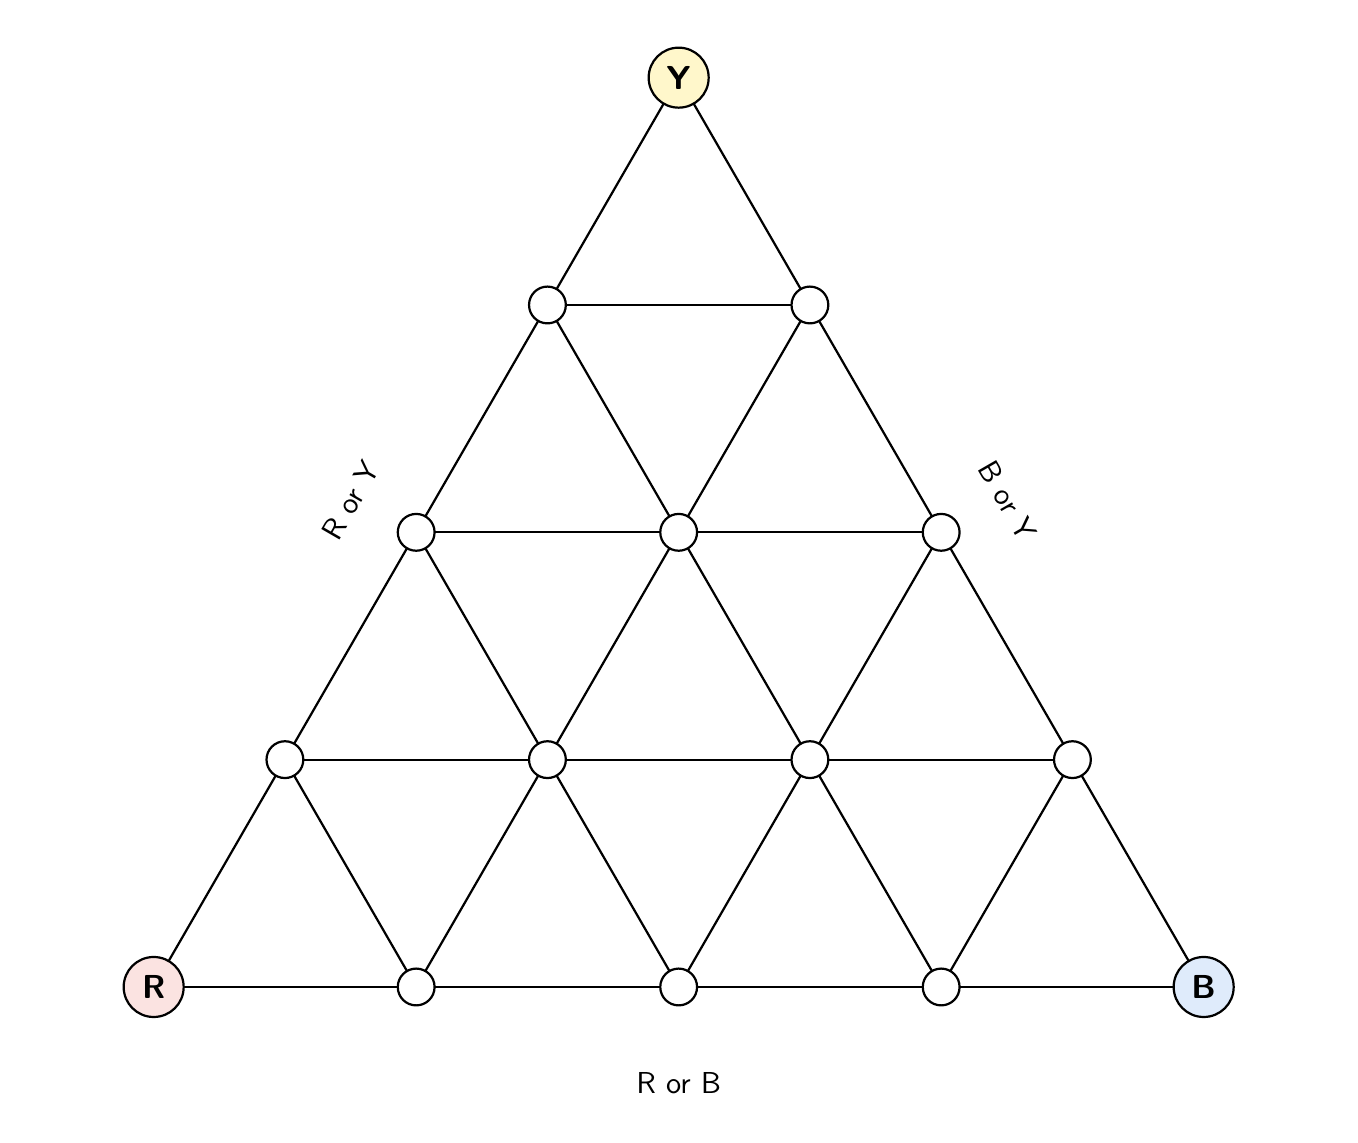
\begin{tikzpicture}[x=1in,y=1in,line cap=round,line join=round]
\path[use as bounding box] (-0.63,-0.64) rectangle (5.8800,4.7966);
\draw[line width=0.8pt] (0.0000,0.0000) -- (0.6562,1.1367);
\draw[line width=0.8pt] (0.0000,0.0000) -- (1.3125,0.0000);
\draw[line width=0.8pt] (0.6562,1.1367) -- (1.3125,2.2733);
\draw[line width=0.8pt] (0.6562,1.1367) -- (1.3125,0.0000);
\draw[line width=0.8pt] (0.6562,1.1367) -- (1.9688,1.1367);
\draw[line width=0.8pt] (1.3125,2.2733) -- (1.9688,3.4100);
\draw[line width=0.8pt] (1.3125,2.2733) -- (1.9688,1.1367);
\draw[line width=0.8pt] (1.3125,2.2733) -- (2.6250,2.2733);
\draw[line width=0.8pt] (1.9688,3.4100) -- (2.6250,4.5466);
\draw[line width=0.8pt] (1.9688,3.4100) -- (2.6250,2.2733);
\draw[line width=0.8pt] (1.9688,3.4100) -- (3.2812,3.4100);
\draw[line width=0.8pt] (2.6250,4.5466) -- (3.2812,3.4100);
\draw[line width=0.8pt] (1.3125,0.0000) -- (1.9688,1.1367);
\draw[line width=0.8pt] (1.3125,0.0000) -- (2.6250,0.0000);
\draw[line width=0.8pt] (1.9688,1.1367) -- (2.6250,2.2733);
\draw[line width=0.8pt] (1.9688,1.1367) -- (2.6250,0.0000);
\draw[line width=0.8pt] (1.9688,1.1367) -- (3.2812,1.1367);
\draw[line width=0.8pt] (2.6250,2.2733) -- (3.2812,3.4100);
\draw[line width=0.8pt] (2.6250,2.2733) -- (3.2812,1.1367);
\draw[line width=0.8pt] (2.6250,2.2733) -- (3.9375,2.2733);
\draw[line width=0.8pt] (3.2812,3.4100) -- (3.9375,2.2733);
\draw[line width=0.8pt] (2.6250,0.0000) -- (3.2812,1.1367);
\draw[line width=0.8pt] (2.6250,0.0000) -- (3.9375,0.0000);
\draw[line width=0.8pt] (3.2812,1.1367) -- (3.9375,2.2733);
\draw[line width=0.8pt] (3.2812,1.1367) -- (3.9375,0.0000);
\draw[line width=0.8pt] (3.2812,1.1367) -- (4.5938,1.1367);
\draw[line width=0.8pt] (3.9375,2.2733) -- (4.5938,1.1367);
\draw[line width=0.8pt] (3.9375,0.0000) -- (4.5938,1.1367);
\draw[line width=0.8pt] (3.9375,0.0000) -- (5.2500,0.0000);
\draw[line width=0.8pt] (4.5938,1.1367) -- (5.2500,0.0000);
\node[circle,draw,line width=0.8pt,fill=Rfill,minimum size=0.30in,inner sep=0pt,font=\sffamily\bfseries\fontsize{11.5}{12}\selectfont] at (0.0000,0.0000) {R};
\draw[line width=0.8pt,fill=white] (1.3125,0.0000) circle[radius=0.092in];
\draw[line width=0.8pt,fill=white] (2.6250,0.0000) circle[radius=0.092in];
\draw[line width=0.8pt,fill=white] (3.9375,0.0000) circle[radius=0.092in];
\node[circle,draw,line width=0.8pt,fill=Bfill,minimum size=0.30in,inner sep=0pt,font=\sffamily\bfseries\fontsize{11.5}{12}\selectfont] at (5.2500,0.0000) {B};
\draw[line width=0.8pt,fill=white] (0.6562,1.1367) circle[radius=0.092in];
\draw[line width=0.8pt,fill=white] (1.9688,1.1367) circle[radius=0.092in];
\draw[line width=0.8pt,fill=white] (3.2812,1.1367) circle[radius=0.092in];
\draw[line width=0.8pt,fill=white] (4.5938,1.1367) circle[radius=0.092in];
\draw[line width=0.8pt,fill=white] (1.3125,2.2733) circle[radius=0.092in];
\draw[line width=0.8pt,fill=white] (2.6250,2.2733) circle[radius=0.092in];
\draw[line width=0.8pt,fill=white] (3.9375,2.2733) circle[radius=0.092in];
\draw[line width=0.8pt,fill=white] (1.9688,3.4100) circle[radius=0.092in];
\draw[line width=0.8pt,fill=white] (3.2812,3.4100) circle[radius=0.092in];
\node[circle,draw,line width=0.8pt,fill=Yfill,minimum size=0.30in,inner sep=0pt,font=\sffamily\bfseries\fontsize{11.5}{12}\selectfont] at (2.6250,4.5466) {Y};
\node[rotate=60,font=\sffamily\fontsize{11}{12}\selectfont] at (0.9825,2.4333) {R or Y};
\node[rotate=-60,font=\sffamily\fontsize{11}{12}\selectfont] at (4.2675,2.4333) {B or Y};
\node[font=\sffamily\fontsize{11}{12}\selectfont] at (2.6250,-0.48) {R or B};
\end{tikzpicture}
\end{center}
\newpage
\textbf{Problem 6:} The bottom side now allows R, B, or Y. Find four different fillings with no little triangle that has R, B, and Y.\par\vspace{0.16in}
\begin{center}
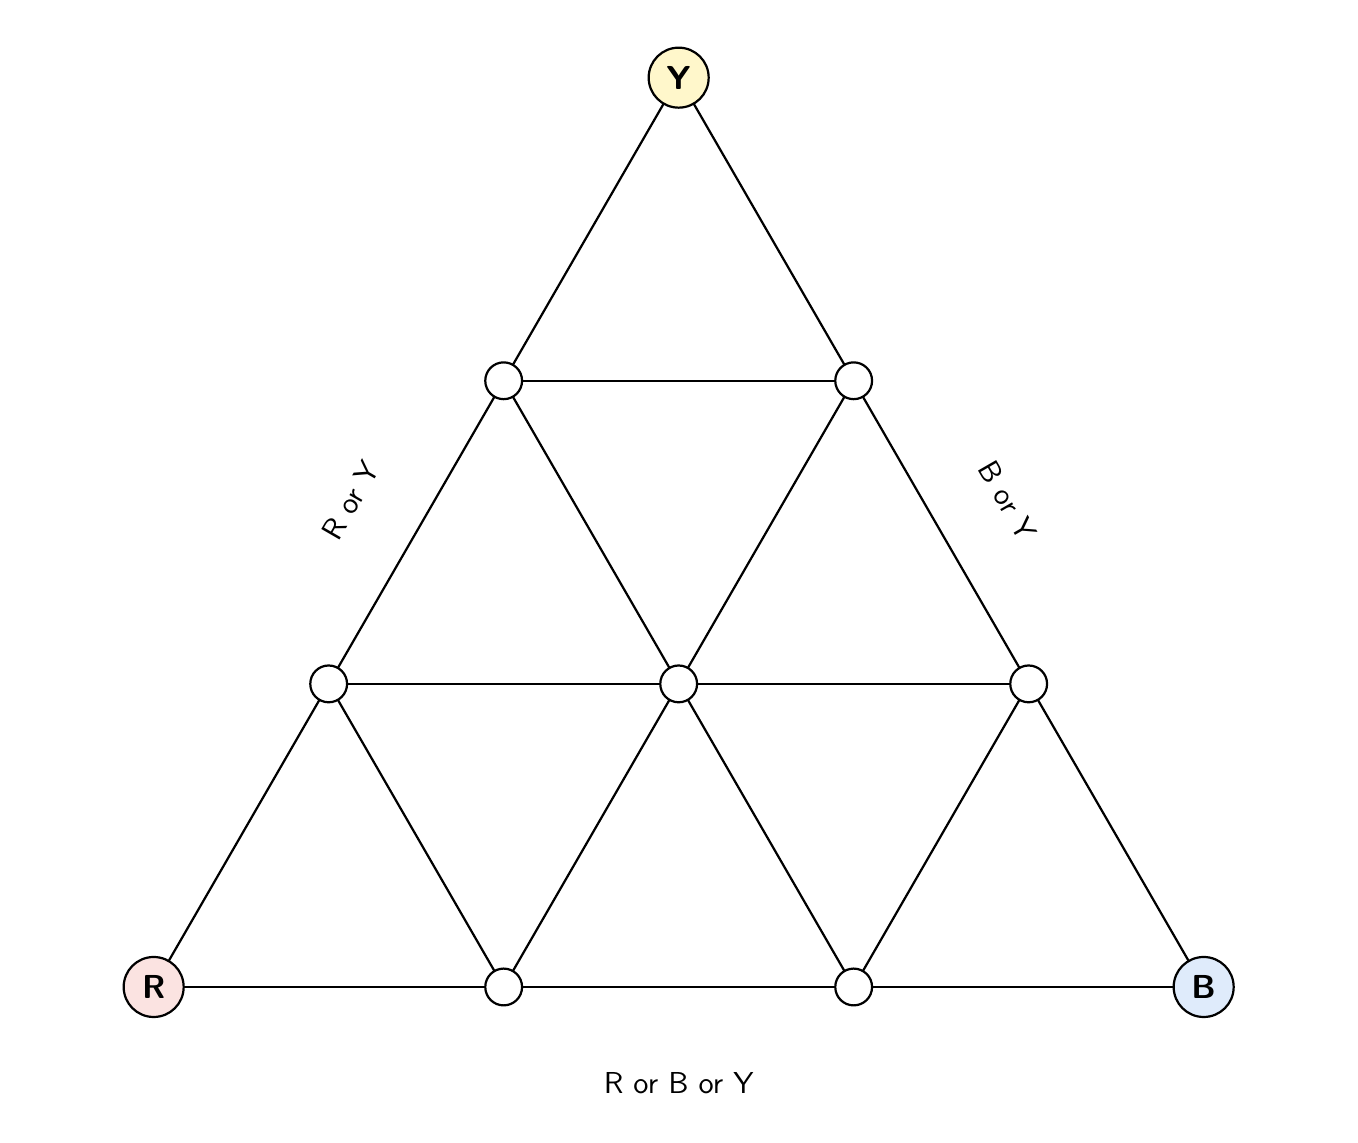
\begin{tikzpicture}[x=1in,y=1in,line cap=round,line join=round]
\path[use as bounding box] (-0.63,-0.64) rectangle (5.8800,4.7966);
\draw[line width=0.8pt] (0.0000,0.0000) -- (0.8750,1.5155);
\draw[line width=0.8pt] (0.0000,0.0000) -- (1.7500,0.0000);
\draw[line width=0.8pt] (0.8750,1.5155) -- (1.7500,3.0311);
\draw[line width=0.8pt] (0.8750,1.5155) -- (1.7500,0.0000);
\draw[line width=0.8pt] (0.8750,1.5155) -- (2.6250,1.5155);
\draw[line width=0.8pt] (1.7500,3.0311) -- (2.6250,4.5466);
\draw[line width=0.8pt] (1.7500,3.0311) -- (2.6250,1.5155);
\draw[line width=0.8pt] (1.7500,3.0311) -- (3.5000,3.0311);
\draw[line width=0.8pt] (2.6250,4.5466) -- (3.5000,3.0311);
\draw[line width=0.8pt] (1.7500,0.0000) -- (2.6250,1.5155);
\draw[line width=0.8pt] (1.7500,0.0000) -- (3.5000,0.0000);
\draw[line width=0.8pt] (2.6250,1.5155) -- (3.5000,3.0311);
\draw[line width=0.8pt] (2.6250,1.5155) -- (3.5000,0.0000);
\draw[line width=0.8pt] (2.6250,1.5155) -- (4.3750,1.5155);
\draw[line width=0.8pt] (3.5000,3.0311) -- (4.3750,1.5155);
\draw[line width=0.8pt] (3.5000,0.0000) -- (4.3750,1.5155);
\draw[line width=0.8pt] (3.5000,0.0000) -- (5.2500,0.0000);
\draw[line width=0.8pt] (4.3750,1.5155) -- (5.2500,0.0000);
\node[circle,draw,line width=0.8pt,fill=Rfill,minimum size=0.30in,inner sep=0pt,font=\sffamily\bfseries\fontsize{11.5}{12}\selectfont] at (0.0000,0.0000) {R};
\draw[line width=0.8pt,fill=white] (1.7500,0.0000) circle[radius=0.092in];
\draw[line width=0.8pt,fill=white] (3.5000,0.0000) circle[radius=0.092in];
\node[circle,draw,line width=0.8pt,fill=Bfill,minimum size=0.30in,inner sep=0pt,font=\sffamily\bfseries\fontsize{11.5}{12}\selectfont] at (5.2500,0.0000) {B};
\draw[line width=0.8pt,fill=white] (0.8750,1.5155) circle[radius=0.092in];
\draw[line width=0.8pt,fill=white] (2.6250,1.5155) circle[radius=0.092in];
\draw[line width=0.8pt,fill=white] (4.3750,1.5155) circle[radius=0.092in];
\draw[line width=0.8pt,fill=white] (1.7500,3.0311) circle[radius=0.092in];
\draw[line width=0.8pt,fill=white] (3.5000,3.0311) circle[radius=0.092in];
\node[circle,draw,line width=0.8pt,fill=Yfill,minimum size=0.30in,inner sep=0pt,font=\sffamily\bfseries\fontsize{11.5}{12}\selectfont] at (2.6250,4.5466) {Y};
\node[rotate=60,font=\sffamily\fontsize{11}{12}\selectfont] at (0.9825,2.4333) {R or Y};
\node[rotate=-60,font=\sffamily\fontsize{11}{12}\selectfont] at (4.2675,2.4333) {B or Y};
\node[font=\sffamily\fontsize{11}{12}\selectfont] at (2.6250,-0.48) {R or B or Y};
\end{tikzpicture}
\end{center}
\end{document}
